\documentclass[runningheads]{llncs}

\usepackage[T1]{fontenc}
\usepackage{graphicx}
\usepackage{booktabs}
\usepackage{multirow}
\usepackage{amsmath}
\usepackage{url}
\usepackage{xcolor}
\usepackage{placeins}
\usepackage{float}

\begin{document}

\title{RT-DETR-L for Road-Scene Object Detection: Ground-Truth Evaluation and Output-Profile Analysis}
\titlerunning{RT-DETR-L Output-Profile Analysis for Road Scenes}

\author{
Lejian Min\inst{1}
\and Ruiqi Guo\inst{1}
\and Zhaolin Dong\inst{1}
}

\authorrunning{L. Min et al.}

\institute{
School of Intelligent Manufacturing Ecosystem,\\
Xi'an Jiaotong-Liverpool University, Suzhou, China
}

\maketitle

\begin{abstract}
Road-scene object detection must remain reliable under changes in object scale, traffic density, occlusion, and illumination. However, aggregate detection scores alone do not explain how pretrained detectors behave in practically difficult scenes or how their outputs change after deployment-oriented filtering. This paper presents a reproducible empirical comparison of pretrained YOLOv8n and RT-DETR-L on \textsc{Road200}, a locked 200-image subset drawn from the BDD100K validation split. The benchmark contains four scenario groups: daytime normal, night low-light, crowded/occluded, and small/distant. Official BDD100K \texttt{box2d} annotations are retained as ground truth, and an explicit shared-category mapping enables class-aware COCO bbox evaluation.

On \textsc{Road200}, RT-DETR-L achieved a higher mAP@[0.50:0.95] than YOLOv8n (0.247 versus 0.127), together with higher AP50, AP75, recall, and F1-score at the selected operating point. YOLOv8n achieved higher precision, indicating a measurable precision--completeness trade-off rather than a uniformly superior detector output. RT-DETR-L showed its largest absolute mAP gains in the crowded/occluded and small/distant scenario groups, while night low-light conditions remained challenging for both models.

A controlled offline ablation of frozen RT-DETR-L predictions further evaluates confidence filtering, maximum retained detections, and external class-aware non-maximum suppression. The results show that output compactness is obtained through an explicit precision--recall trade-off, not through a free improvement in underlying detection capability. The paper therefore distinguishes raw AP-ranking predictions from balanced and compact deployment-oriented output profiles.
\end{abstract}

\keywords{Road-scene object detection \and RT-DETR-L \and YOLOv8n \and COCO evaluation \and post-processing \and BDD100K}

\section{Introduction}

Object detection is a core component of camera-based road-scene perception. Vehicles, pedestrians, bicycles, traffic lights, and other road-relevant objects must be located before later modules can perform risk estimation, tracking, warning, or planning. However, road scenes are not homogeneous detection environments. Object scale, traffic density, partial occlusion, illumination, and background clutter can change substantially between images, making an overall detection score insufficient for explaining how a pretrained detector behaves in practically difficult conditions.

Modern object detectors include two-stage CNN detectors, one-stage dense detectors, anchor-free methods, and Transformer-based set-prediction models~\cite{zou2023survey,ren2015faster,wang2024yolov10}. Lightweight YOLO models remain common engineering baselines because they provide practical one-stage inference through a mature deployment ecosystem. In parallel, DETR reformulated object detection as direct set prediction using learned object queries and bipartite matching~\cite{carion2020detr}. Deformable DETR improved the original formulation by using sparse deformable attention, addressing slow convergence and improving the handling of multi-scale features and small objects~\cite{zhu2021deformable}. RT-DETR subsequently adapted the DETR family to real-time detection through an efficient hybrid encoder and query-selection design~\cite{zhao2024detrsbeat}, while RT-DETRv2 explored further training and deployment-oriented refinements~\cite{lv2024rtdetrv2}.

Although pretrained detector comparisons are often reported through aggregate AP values, practical road-scene use requires two related but distinct questions. The first is whether the detector correctly localises and classifies objects under a standard ground-truth evaluation protocol. The second is how the retained output behaves at a chosen operating point. A raw ranked prediction set may be suitable for AP calculation but may contain many low-confidence or overlapping candidates that are difficult to inspect directly. Conversely, a compact displayed output may be easier to read but can reduce recall by removing valid candidate detections. These objectives should therefore be evaluated separately rather than treating visually cleaner output as automatic evidence of higher detection accuracy.

This paper studies this distinction using \textsc{Road200}, a locked 200-image road-scene evaluation subset drawn exclusively from the BDD100K validation split~\cite{yu2020bdd100k}. The benchmark contains four scenario groups: daytime normal, night low-light, crowded/occluded, and small/distant. Official BDD100K \texttt{box2d} annotations are retained as ground truth, and an explicit mapping is used to evaluate the COCO-compatible shared categories of the pretrained models. COCO-style class-aware bbox evaluation is then used to report mAP@[0.50:0.95], AP50, AP75, precision, recall, and F1-score~\cite{lin2014coco}.

The empirical comparison focuses on pretrained YOLOv8n and RT-DETR-L. YOLOv8n serves as a lightweight engineering baseline, whereas RT-DETR-L represents a real-time DETR-family detector. The study does not fine-tune either model and does not propose a new detector architecture. Instead, it evaluates whether the measured detector comparison changes across road-scene scenarios and how RT-DETR-L output density can be adjusted through confidence filtering, maximum-output capping, and external class-aware non-maximum suppression (NMS).

The contributions of this paper are as follows:

\begin{itemize}
\item A locked, manifest-defined 200-image road-scene evaluation subset derived from the BDD100K validation split, organised into four scenario groups and paired with official \texttt{box2d} ground-truth annotations.

\item A class-aware evaluation protocol that compares pretrained YOLOv8n and RT-DETR-L using standard COCO bbox metrics together with a fixed operating-point precision--recall--F1 analysis.

\item A controlled offline ablation of confidence thresholds, maximum retained detections, and external class-aware NMS on frozen RT-DETR-L predictions, separating raw AP-ranking output from deployment-oriented output profiles.

\item A deterministic qualitative analysis protocol that selects representative scenario cases using benchmark statistics rather than manual cherry-picking.

\end{itemize}

The results show that RT-DETR-L achieves stronger class-aware COCO detection metrics than YOLOv8n on the locked \textsc{Road200} benchmark, while YOLOv8n provides higher precision at the selected operating threshold. The post-processing analysis further shows that output compactness is obtained through an explicit recall--precision trade-off rather than a free improvement in underlying detection capability.

The remainder of this paper is organised as follows. Section~2 reviews road-scene detection, DETR-family methods, and relevant benchmark datasets. Section~3 describes \textsc{Road200}, the model configurations, and the evaluation protocol. Section~4 presents the automatic evaluation, scenario-level analysis, output-level ablation, and qualitative cases. Section~5 discusses the implications and limitations of the findings, and Section~6 concludes the paper.

\section{Related Work}

\subsection{Road-scene Object Detection and Efficient Baselines}

Road-scene object detection requires simultaneous handling of large vehicles, small pedestrians, traffic lights, partial occlusion, background clutter, and changes in illumination. Modern detectors are commonly described through two-stage, one-stage, anchor-free, and end-to-end set-prediction designs~\cite{zou2023survey}. These lines of work differ not only in architecture but also in how they balance localization, object coverage, computational cost, and output post-processing.

Two-stage detectors such as Faster R-CNN generate candidate regions before classification and bounding-box refinement~\cite{ren2015faster}. This approach established a strong accuracy-oriented reference, but its multi-stage structure can be less convenient when low-latency inference is important. In contrast, one-stage detectors directly predict object categories and locations from dense image features. Recent real-time methods such as YOLOv10 aim to improve the efficiency--accuracy balance of this design~\cite{wang2024yolov10}. In the present study, YOLOv8n is used as a lightweight engineering baseline rather than as a representative of every YOLO variant.

Anchor-free methods provide a related perspective. FCOS formulates detection as per-pixel prediction without predefined anchor boxes~\cite{tian2019fcos}, whereas ATSS analyses the selection of positive and negative training samples across anchor-based and anchor-free detectors~\cite{zhang2020atss}. These studies are relevant because road scenes often contain objects with substantial scale variation. However, they also show that detector behaviour cannot be reduced to a single architectural label. Training assignment, feature representation, confidence scoring, and post-processing all influence the final retained outputs.

For this work, the role of YOLOv8n is therefore deliberately limited. It provides a lightweight pretrained baseline against which the class-aware detection performance and output-level behaviour of RT-DETR-L can be compared on the same locked Road200 benchmark.

\subsection{DETR-family Detection and Output-level Refinement}

DETR introduced an end-to-end formulation of object detection as direct set prediction~\cite{carion2020detr}. Instead of relying on proposal generation and conventional detector-native non-maximum suppression, DETR uses learned object queries and bipartite matching between predictions and ground-truth objects. This design is important for the present study because it means that the raw ranked output of a DETR-family model should not automatically be interpreted through the same pipeline assumptions used by conventional dense detectors.

The original DETR nevertheless had recognised limitations, including slow convergence and weaker performance for small objects. Deformable DETR addressed these issues through sparse deformable attention over a limited set of relevant sampling points across feature maps~\cite{zhu2021deformable}. RT-DETR subsequently adapted the DETR family toward real-time object detection through an efficient hybrid encoder, multi-scale processing, and query-selection design~\cite{zhao2024detrsbeat}. RT-DETRv2 further explored training and deployment-oriented refinements, including multi-scale sampling flexibility and changes intended to improve practical deployment~\cite{lv2024rtdetrv2}.

These studies motivate the use of RT-DETR-L as a Transformer-based comparison model, but they do not imply that a pretrained RT-DETR-L output is universally optimal for every downstream use. Standard COCO AP evaluates ranked detections against ground truth, whereas a practical road-scene interface must also manage output density, overlapping candidate boxes, and the trade-off between precision and recall at a chosen operating threshold.

Non-maximum suppression is relevant to this distinction. In conventional detection pipelines, NMS suppresses overlapping candidates and therefore introduces a recall--precision trade-off governed by a suppression threshold~\cite{hosang2017learningnms}. In contrast, the native DETR formulation is designed to predict a final set without conventional NMS~\cite{carion2020detr}. Accordingly, this paper does not describe NMS as a required RT-DETR-L component. Instead, it evaluates \emph{external class-aware NMS} as an explicit output-layer intervention applied to frozen RT-DETR-L predictions. Its purpose is to test whether redundant displayed outputs can be reduced while maintaining useful detection behaviour under the same ground-truth evaluation protocol.

\subsection{Road-scene Datasets and the Position of Road200}

Road-scene datasets differ in sensing modality, annotation format, scale, and intended task. BDD100K provides geographically and visually diverse driving data with heterogeneous labels across multiple perception tasks~\cite{yu2020bdd100k}. Waymo Open Dataset provides synchronized camera and LiDAR data with 2D and 3D annotations~\cite{sun2020waymo}, while Argoverse 2 extends the available self-driving data resources for multimodal perception and forecasting~\cite{wilson2023argoverse2}. These datasets support broader autonomous-driving research, but they are not interchangeable for a focused 2D pretrained-detector case study.

Microsoft COCO remains important because its object taxonomy and evaluation protocol are widely used to train and assess general object detectors~\cite{lin2014coco}. In this paper, COCO is not treated as an image source. Instead, it provides the pretrained detector label space and the standard bbox evaluation protocol used for class-aware AP calculation.

Road200 is positioned as a reproducible, scenario-oriented evaluation subset rather than a new large-scale dataset. It is drawn exclusively from the BDD100K validation split, with official BDD100K \texttt{box2d} annotations retained as ground truth. The benchmark isolates four practical road-scene conditions---daytime normal, night low-light, crowded/occluded, and small/distant---while using a fixed manifest and an explicit BDD100K-to-COCO category mapping. This design does not claim to replace large driving benchmarks. Its purpose is to provide a controlled case-study setting in which automatic detection metrics, output-density ablations, and deterministic qualitative examples can be interpreted together.

\FloatBarrier

\section{Methodology}

\subsection{Research Design}

This work adopts a controlled empirical case-study design to compare a lightweight CNN-based detector, YOLOv8n, with the Transformer-based RT-DETR-L detector on a fixed road-scene benchmark. The study has two linked objectives. First, it establishes a class-aware detection baseline using official BDD100K bounding-box annotations and standard COCO metrics. Second, it investigates whether explicit output-layer strategies can improve the practical readability of RT-DETR-L predictions without obscuring their accuracy--completeness trade-off.

The principal evidence is automatic and ground-truth-based: COCO average precision, class-aware operating-point precision, recall, and F1-score. Qualitative inspection is used only as supplementary diagnostic evidence. It is not used to assign the primary model ranking or to replace standard detection metrics. This distinction is important because visually cleaner outputs do not necessarily imply higher detection accuracy.

\subsection{Road200 Benchmark and Scenario Construction}

All evaluation images were drawn from the validation split of BDD100K~\cite{yu2020bdd100k}. The final benchmark, denoted as \textsc{Road200}, contains 200 images divided equally into four scenario groups:

\begin{itemize}
\item \textbf{Daytime normal:} daytime road scenes without an explicit difficulty constraint;
\item \textbf{Night low-light:} scenes recorded under night-time illumination;
\item \textbf{Crowded or occluded:} scenes containing dense road users and/or substantial object overlap;
\item \textbf{Small or distant:} scenes in which road-relevant objects occupy relatively small image regions or appear at long range.
\end{itemize}

Scenario-specific candidate filters were first applied to BDD100K metadata and object annotations. A fixed random seed was then used to form a candidate pool of 70 images for each scenario. The candidate images were reviewed at full resolution using predefined inclusion and exclusion criteria, after which 50 images were retained for each group. The resulting manifest records the original BDD100K image identifier, scenario label, image path, and corresponding annotation path. This manifest, together with the construction records and evaluation scripts, provides the image index required to reproduce the locked \textsc{Road200} subset.

The original BDD100K \texttt{box2d} annotations were used directly as ground truth; no bounding boxes were manually redrawn. To ensure a fair comparison with COCO-pretrained detectors, the evaluation retained only categories with a clear BDD100K-to-COCO correspondence. The final evaluation schema contains eight categories, shown in Table~\ref{tab:road200_class_mapping}. BDD categories such as \texttt{traffic sign}, \texttt{rider}, lane markings, and drivable-area annotations were excluded because they do not provide a clean one-to-one comparison with the COCO output taxonomy.

\begin{table}[t]
\caption{BDD100K-to-COCO category mapping used in the \textsc{Road200} evaluation.}
\label{tab:road200_class_mapping}
\centering
\small
\begin{tabular}{lll}
\hline
BDD100K category & Evaluation category & COCO-pretrained output \\
\hline
\texttt{person}        & person        & person \\
\texttt{bike}          & bicycle       & bicycle \\
\texttt{car}           & car           & car \\
\texttt{motor}         & motorcycle    & motorcycle \\
\texttt{bus}           & bus           & bus \\
\texttt{train}         & train         & train \\
\texttt{truck}         & truck         & truck \\
\texttt{traffic light} & traffic light & traffic light \\
\hline
\end{tabular}
\end{table}

The locked benchmark contains 3067 ground-truth boxes in the shared evaluation taxonomy. A further 761 BDD100K bounding-box annotations were excluded because they belonged to unmapped categories. Figure~\ref{fig:road200_examples} presents one fixed representative image from each scenario. The displayed images are selected from the same reproducibility-controlled case-selection record used later for qualitative analysis; they are not manually chosen to favour either detector.

\begin{figure}[t]
\centering
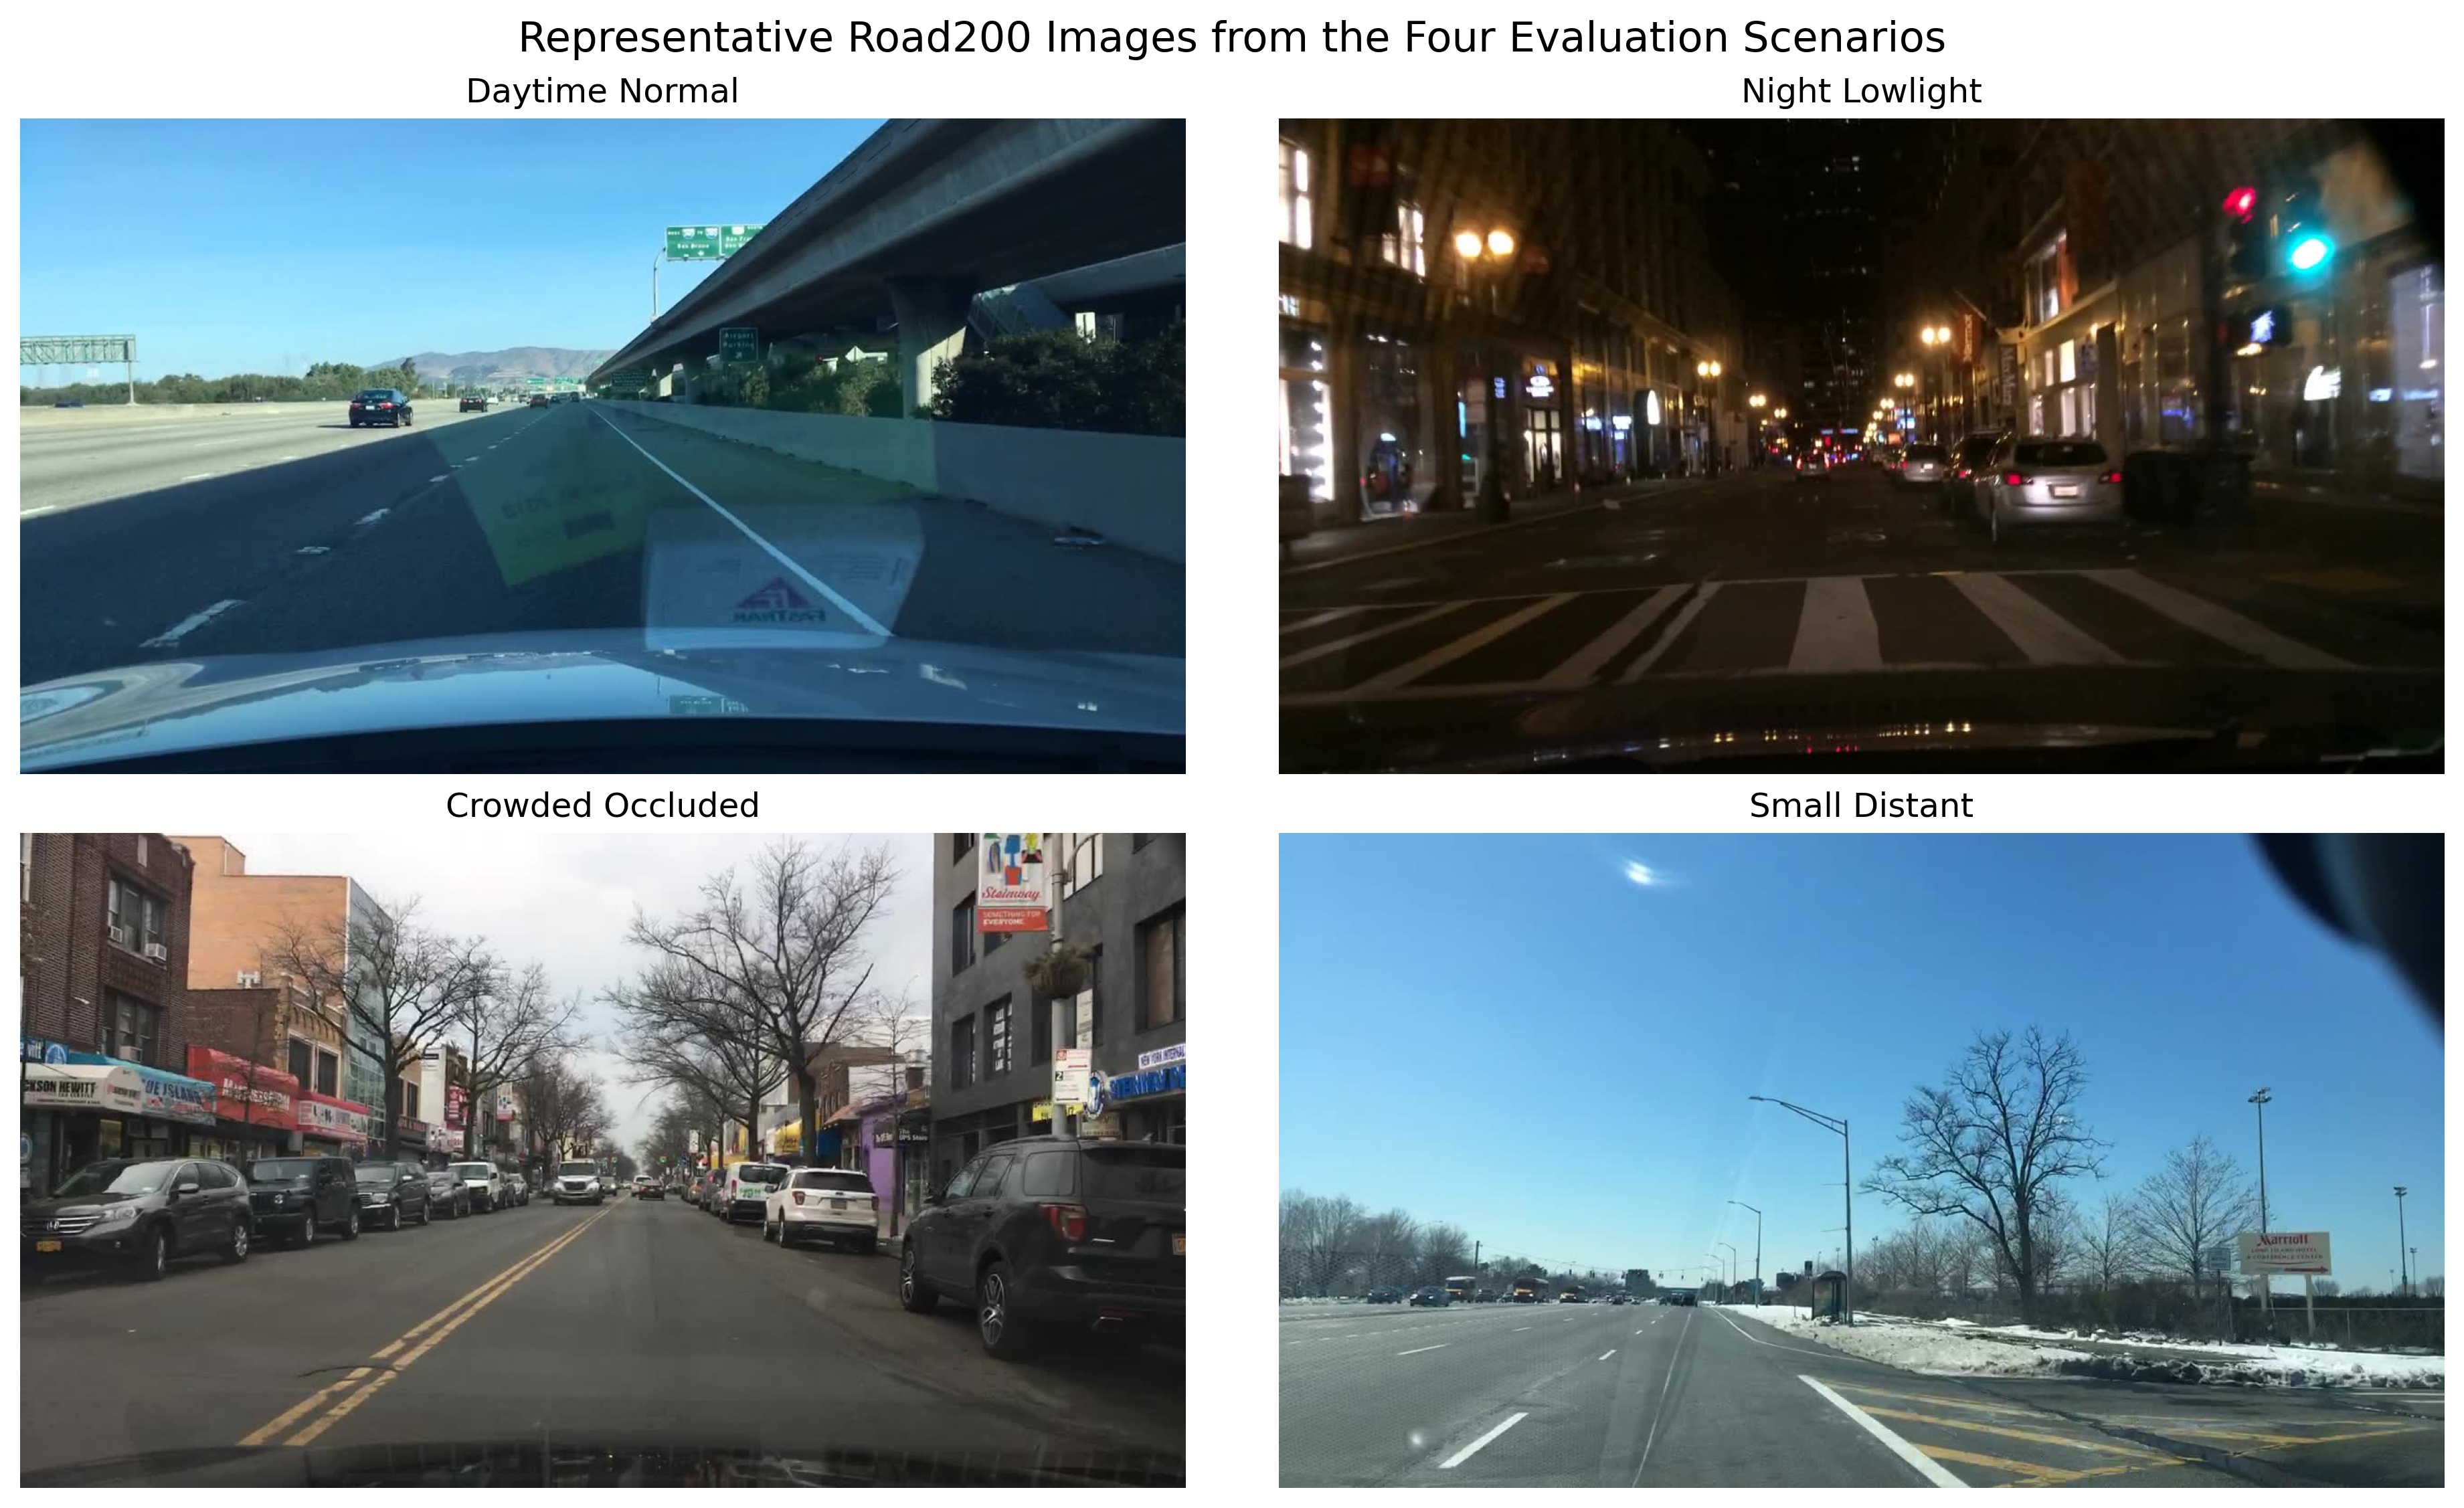
\includegraphics[width=0.96\textwidth]{figures/road200_scenario_examples.png}
\caption{Representative images from the four locked \textsc{Road200} evaluation scenarios.}
\label{fig:road200_examples}
\end{figure}

\subsection{Detection Models}

Two publicly available COCO-pretrained detectors were evaluated without additional fine-tuning on \textsc{Road200}.

\textbf{YOLOv8n} was selected as a lightweight reference detector. Its small model scale and accessible deployment workflow make it a suitable baseline for practical road-scene inference~\cite{ultralytics2023yolov8}. YOLOv8n was not modified beyond the inference settings required by the standard evaluation pipeline.

\textbf{RT-DETR-L} was selected as the Transformer-based comparison model. DETR-style detection formulates object detection as a set-prediction problem rather than relying on conventional proposal generation and detector-native non-maximum suppression~\cite{carion2020detr}. RT-DETR extends this family toward real-time detection~\cite{zhao2024detrsbeat}, while RT-DETRv2 provides a related improved baseline~\cite{lv2024rtdetrv2}. In this study, RT-DETR-L is not presented as a newly trained or modified architecture. Instead, its frozen prediction outputs are analysed under explicit post-processing configurations.

Both detectors were evaluated at an image size of 640 pixels. Predictions outside the eight shared classes in Table~\ref{tab:road200_class_mapping} were excluded before automatic matching. A prediction could match a ground-truth object only when its mapped class label was identical and its bounding-box overlap satisfied the relevant IoU criterion.

\subsection{RT-DETR-L Output-Refinement Profiles}

The post-processing study operates on frozen, confidence-ranked RT-DETR-L predictions. Its purpose is not to claim that RT-DETR-L intrinsically requires NMS. Instead, external class-aware NMS is treated as a controlled output-layer intervention for examining whether redundant predictions can be reduced while preserving practically useful detections.

For a prediction set $\mathcal{P}$, a profile is defined by a confidence floor $\tau$, an optional external class-aware NMS threshold $\eta$, and a global per-image top-$K$ constraint:

\[
\mathcal{P}_{\tau,\eta,K}
=
\mathrm{TopK}_{K}
\left(
\mathrm{NMS}_{\eta}
\left(
\left\{
p \in \mathcal{P}
\mid
s(p) \geq \tau
\right\}
\right)
\right).
\]

When external NMS is enabled, suppression is performed only between predictions from the same image and the same predicted class. The processing order is therefore: confidence filtering, optional class-aware NMS, and global top-$K$ retention per image. Visualization is applied only after metric evaluation and does not alter any reported detection score.

Three profiles are retained for the final analysis. The raw metric baseline preserves low-confidence ranked predictions for COCO AP calculation. The balanced profile prioritizes recall and readable outputs, whereas the compact profile prioritizes precision, F1-score, and reduced output density.

\begin{table}[t]
\caption{Frozen RT-DETR-L output profiles used in the final analysis. External NMS denotes an added class-aware output-layer operation rather than a native RT-DETR-L component.}
\label{tab:rtdetr_profiles}
\centering
\small
\begin{tabular}{lccc}
\hline
Profile & Confidence floor & External NMS IoU & Top-$K$ \\
\hline
Raw metric baseline & 0.001 & None & 300 \\
Balanced output profile & 0.25 & 0.45 & 100 \\
Compact output profile & 0.35 & 0.55 & 100 \\
\hline
\end{tabular}
\end{table}

Figure~\ref{fig:road200_workflow} summarizes the complete benchmark, evaluation, and output-refinement workflow. The standard detector comparison and the RT-DETR-L output-profile analysis share the same locked images, mapped ground truth, and COCO evaluation protocol.

\begin{figure}[t]
\centering
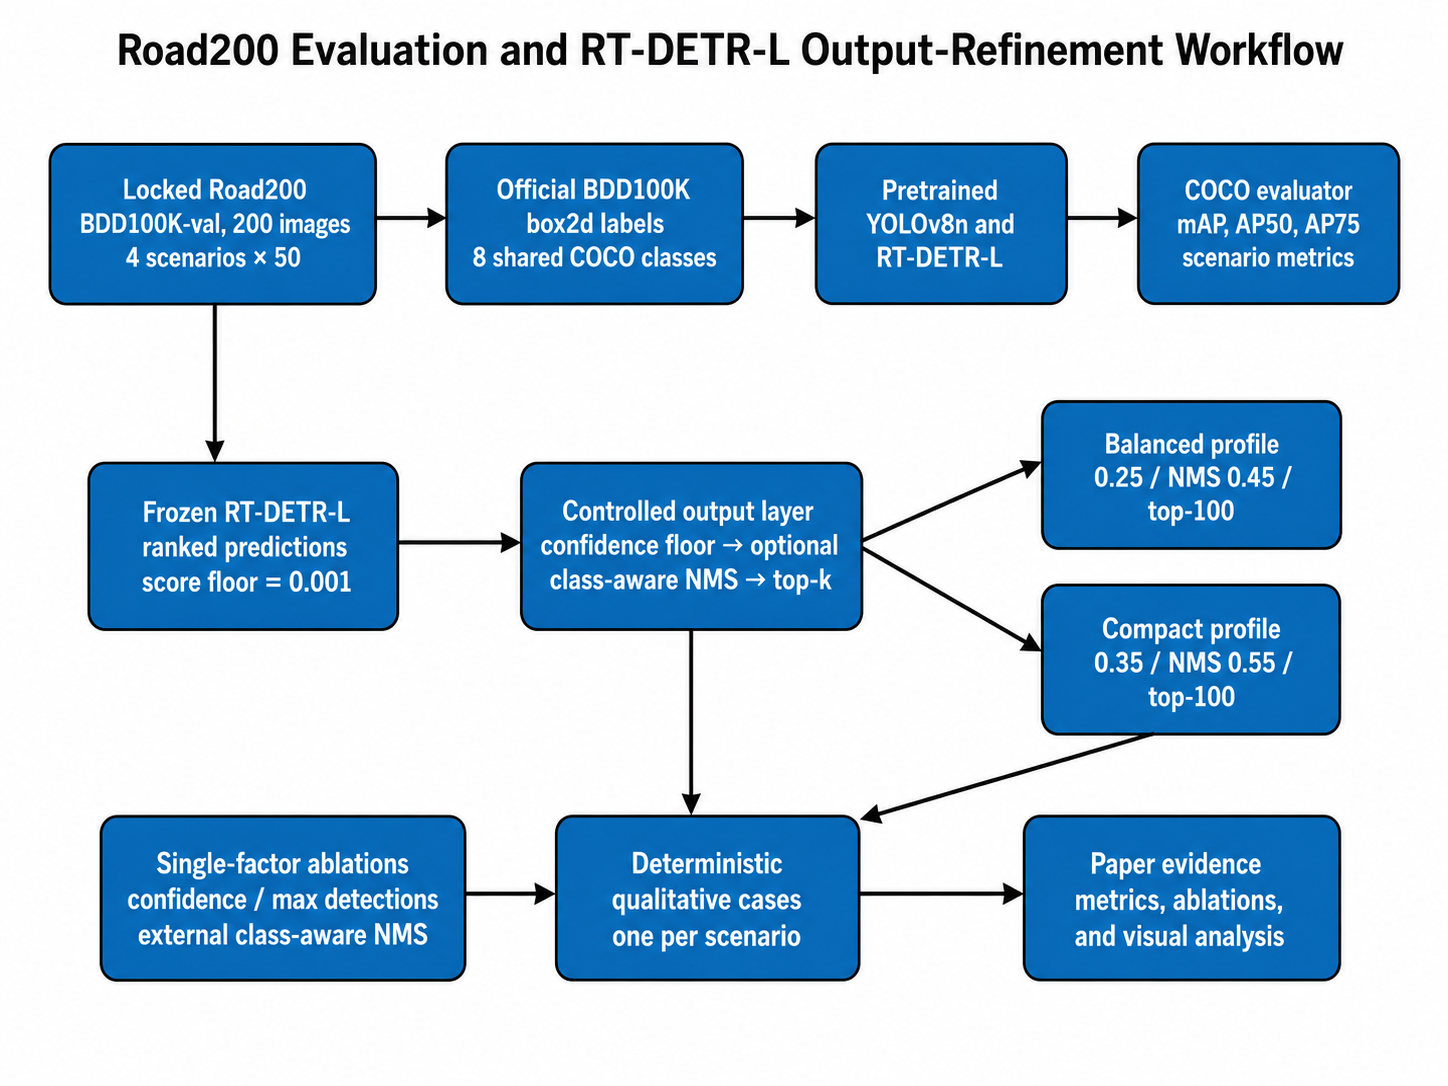
\includegraphics[width=0.98\textwidth]{figures/road200_evaluation_pipeline.png}
\caption{Road200 evaluation and RT-DETR-L output-refinement workflow. The external class-aware NMS stage is an experimental post-processing intervention, not a native RT-DETR-L requirement.}
\label{fig:road200_workflow}
\end{figure}

\subsection{Evaluation Protocol}

Automatic detection evaluation follows the COCO bounding-box protocol~\cite{lin2014coco}. The primary metric is mAP@[0.50:0.95], calculated across IoU thresholds from 0.50 to 0.95 in increments of 0.05. AP50 and AP75 are also reported to distinguish looser and stricter localization requirements. All COCO metrics are calculated with the official \texttt{pycocotools} bbox evaluator using the eight shared categories and the standard maximum-detection setting of 100.

The raw metric baseline uses an inference score floor of 0.001 so that ranked low-confidence predictions remain available for AP calculation. This low floor is not interpreted as an operational deployment threshold. For a directly interpretable operating point, class-aware precision, recall, and F1-score are separately calculated at confidence $0.25$ and IoU $0.50$. Each prediction is matched at most once to a ground-truth box of the same mapped category.

Scenario-level metrics are calculated independently for the four 50-image groups. Class-level AP is reported only for classes represented in the locked subset; categories with no ground-truth instances are marked as not applicable rather than assigned an artificial score of zero.

A systematic RT-DETR-L ablation study examines three factors: confidence floors of $0.001$, $0.05$, $0.10$, $0.20$, $0.25$, $0.35$, and $0.50$; per-image maximum detections of 50, 100, and 300; and external class-aware NMS IoU thresholds of none, $0.45$, $0.55$, and $0.65$. Single-factor studies are first conducted using the same frozen prediction set. A subsequent composed-profile study validates the balanced and compact configurations in Table~\ref{tab:rtdetr_profiles}.

Qualitative inspection is supplementary. One representative image per scenario is selected deterministically using the scenario median of three quantities: the number of shared-class ground-truth boxes, balanced-profile retained detections, and compact-profile retained detections. This avoids manually selecting visually favourable examples. Manual observations may be used to describe error types, such as missed small objects or redundant candidate boxes, but no manually assigned usefulness score is used as a principal performance metric.

\FloatBarrier

\section{Experiments and Results}

\subsection{Experimental Setup}

The standard \textsc{Road200} evaluation was conducted in the
\texttt{road\_det\_bdd} Conda environment on a Windows 11 laptop
equipped with an NVIDIA RTX 5080 Laptop GPU with 15.92\,GiB of
available VRAM. The software stack used Python 3.10.20, PyTorch 2.11.0 with CUDA 12.8 support, and Ultralytics 8.4.78. Both pretrained detectors were evaluated at an input size of $640 \times 640$ pixels.

The automatic evaluation used the locked 200-image \textsc{Road200} benchmark and its official BDD100K \texttt{box2d} ground-truth annotations. COCO AP metrics were calculated from ranked predictions retained with an inference score floor of 0.001. By contrast, the operating-point precision, recall, and F1-score values reported below use a confidence threshold of 0.25 and class-aware one-to-one matching at IoU $=0.50$.

Because the standardized evaluation loop includes image loading, model prediction, prediction conversion, and metric export, it is not used as a dedicated latency benchmark. Accordingly, this paper reports no cross-model FPS comparison. Therefore, its measured wall-clock time is not reported as a standalone FPS benchmark. The earlier exploratory FPS values obtained on a different hardware platform are not directly comparable with the current standardized Road200 evaluation and are not used as primary evidence.

\begin{table}[H]
\caption{Hardware, software, and evaluation configuration for the standardized Road200 experiments.}
\label{tab:experimental_setup}
\centering
\small
\begin{tabular}{ll}
\hline
Component & Configuration \\
\hline
Operating system & Windows 11 \\
GPU & NVIDIA RTX 5080 Laptop GPU, 15.92\,GiB VRAM \\
Python & 3.10.20 \\
PyTorch & 2.11.0 with CUDA 12.8 support \\
Ultralytics & 8.4.78 \\
Input resolution & $640 \times 640$ \\
Primary evaluator & \texttt{pycocotools} COCO bbox evaluator \\
COCO IoU thresholds & $0.50$ to $0.95$ in increments of $0.05$ \\
Operating-point matching & confidence $=0.25$, IoU $=0.50$ \\
\hline
\end{tabular}
\end{table}

\subsection{Overall Class-aware Detection Performance}

Table~\ref{tab:overall_coco_results} presents the primary automatic comparison. RT-DETR-L achieved higher mAP@[0.50:0.95], AP50, and AP75 than YOLOv8n. In particular, RT-DETR-L improved mAP@[0.50:0.95] from 0.127 to 0.247 and AP50 from 0.221 to 0.456.

At the fixed operating point, YOLOv8n obtained higher precision, whereas RT-DETR-L achieved substantially higher recall and F1-score. This result describes a measurable trade-off on the locked benchmark: YOLOv8n produced a more conservative output at confidence 0.25, while RT-DETR-L recovered more ground-truth objects and obtained the stronger balanced operating-point score.

\begin{table}[H]
\caption{Overall class-aware detection performance on the locked \textsc{Road200} benchmark. AP metrics are calculated using ranked predictions and the official COCO bbox evaluator. P, R, and F1 are calculated at confidence $=0.25$ and IoU $=0.50$.}
\label{tab:overall_coco_results}
\centering
\small
\begin{tabular}{lrrrrrr}
\hline
Model & mAP & AP50 & AP75 & P & R & F1 \\
\hline
YOLOv8n & 0.127 & 0.221 & 0.120 & \textbf{0.718} & 0.315 & 0.438 \\
RT-DETR-L & \textbf{0.247} & \textbf{0.456} & \textbf{0.231} & 0.531 & \textbf{0.608} & \textbf{0.567} \\
\hline
\end{tabular}
\end{table}

The class-level results provide additional evidence for the aggregate comparison. For the dominant \texttt{car} class, which accounts for 2234 of the 3067 shared-class ground-truth boxes, RT-DETR-L obtained an AP@[0.50:0.95] of 0.385 compared with 0.284 for YOLOv8n. RT-DETR-L also achieved higher AP on \texttt{traffic light} (0.132 versus 0.043), \texttt{person} (0.227 versus 0.132), \texttt{truck} (0.297 versus 0.179), and \texttt{bus} (0.251 versus 0.146). These smaller categories should be interpreted cautiously because their instance counts are limited. The \texttt{train} category had no ground-truth instance in the locked subset and is therefore treated as not applicable in class-wise reporting rather than assigned an artificial score of zero.

\begin{figure}[!htbp]
\centering
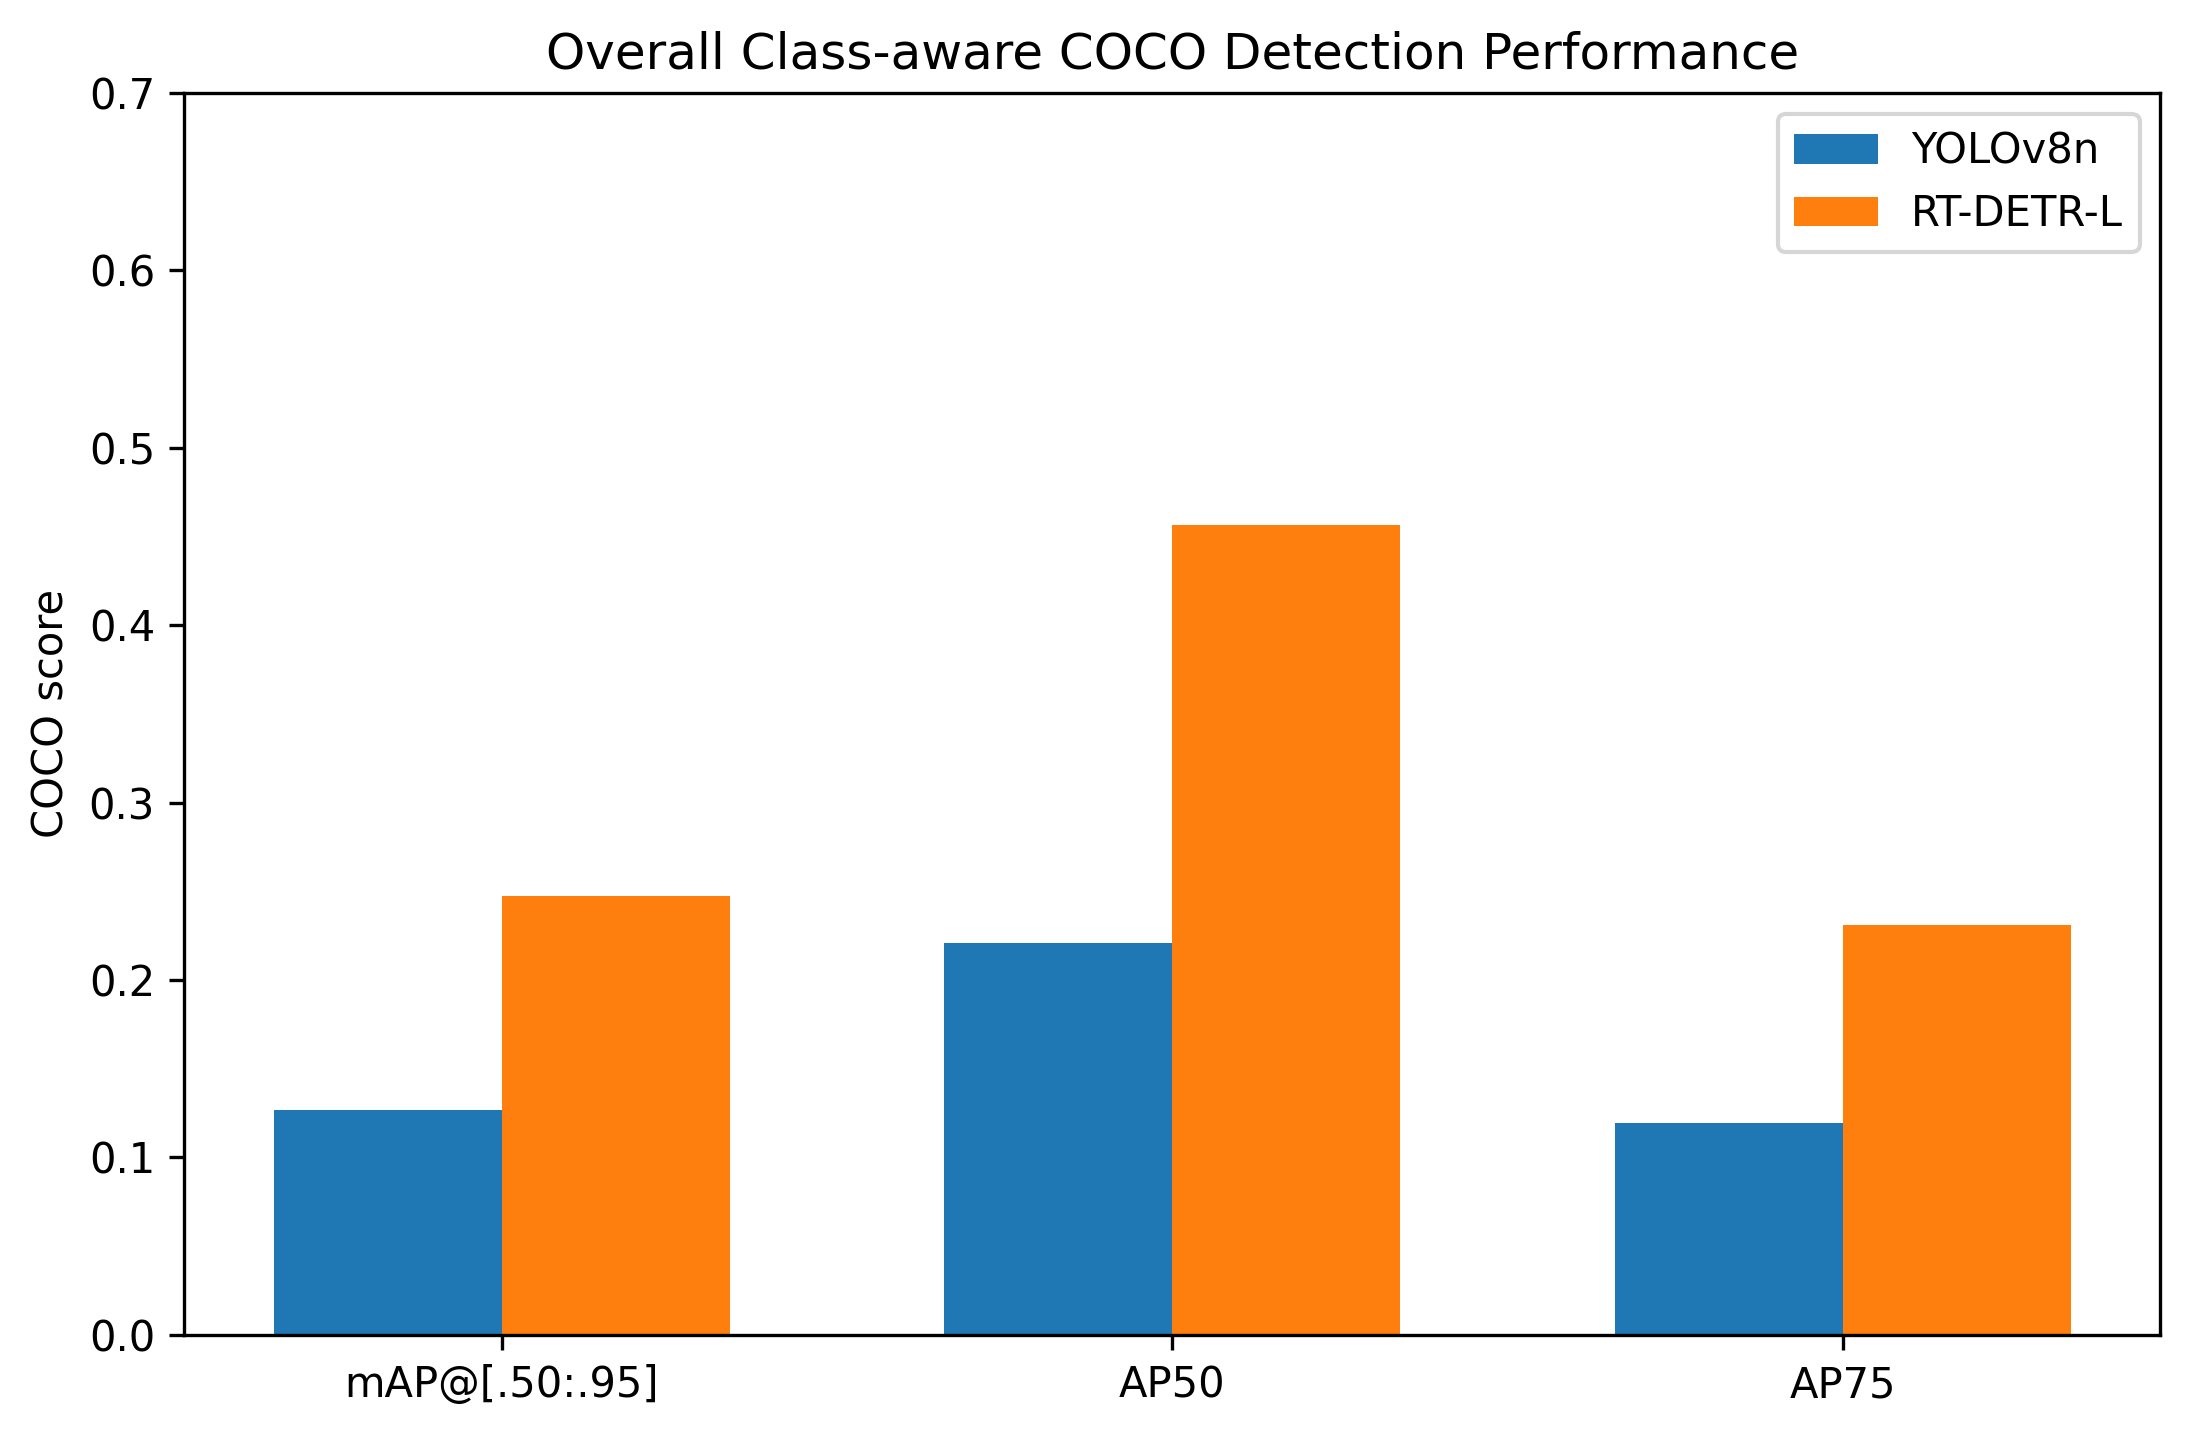
\includegraphics[width=0.78\textwidth]{figures/road200_overall_ap_comparison.png}
\caption{Overall class-aware COCO AP comparison on \textsc{Road200}. RT-DETR-L achieved higher mAP@[0.50:0.95], AP50, and AP75 than YOLOv8n.}
\label{fig:overall_ap_comparison}
\end{figure}

\FloatBarrier

\subsection{Scenario-wise Performance}

Table~\ref{tab:scenario_results} reports the scenario-level breakdown. Daytime normal scenes were the strongest condition for both models, whereas night low-light scenes were the weakest condition in terms of mAP. RT-DETR-L outperformed YOLOv8n in all four groups.

The largest absolute mAP advantage for RT-DETR-L occurred in the small/distant scenario, where the score increased from 0.091 to 0.222. The crowded/occluded scenario showed a similarly large increase from 0.151 to 0.281. These results show that the relative advantage of RT-DETR-L on this benchmark is most pronounced in scenarios containing small targets, partial visibility, or dense object layouts. However, the night low-light results also show that both models remain substantially less effective under difficult illumination.

\begin{figure}[!htbp]
\centering
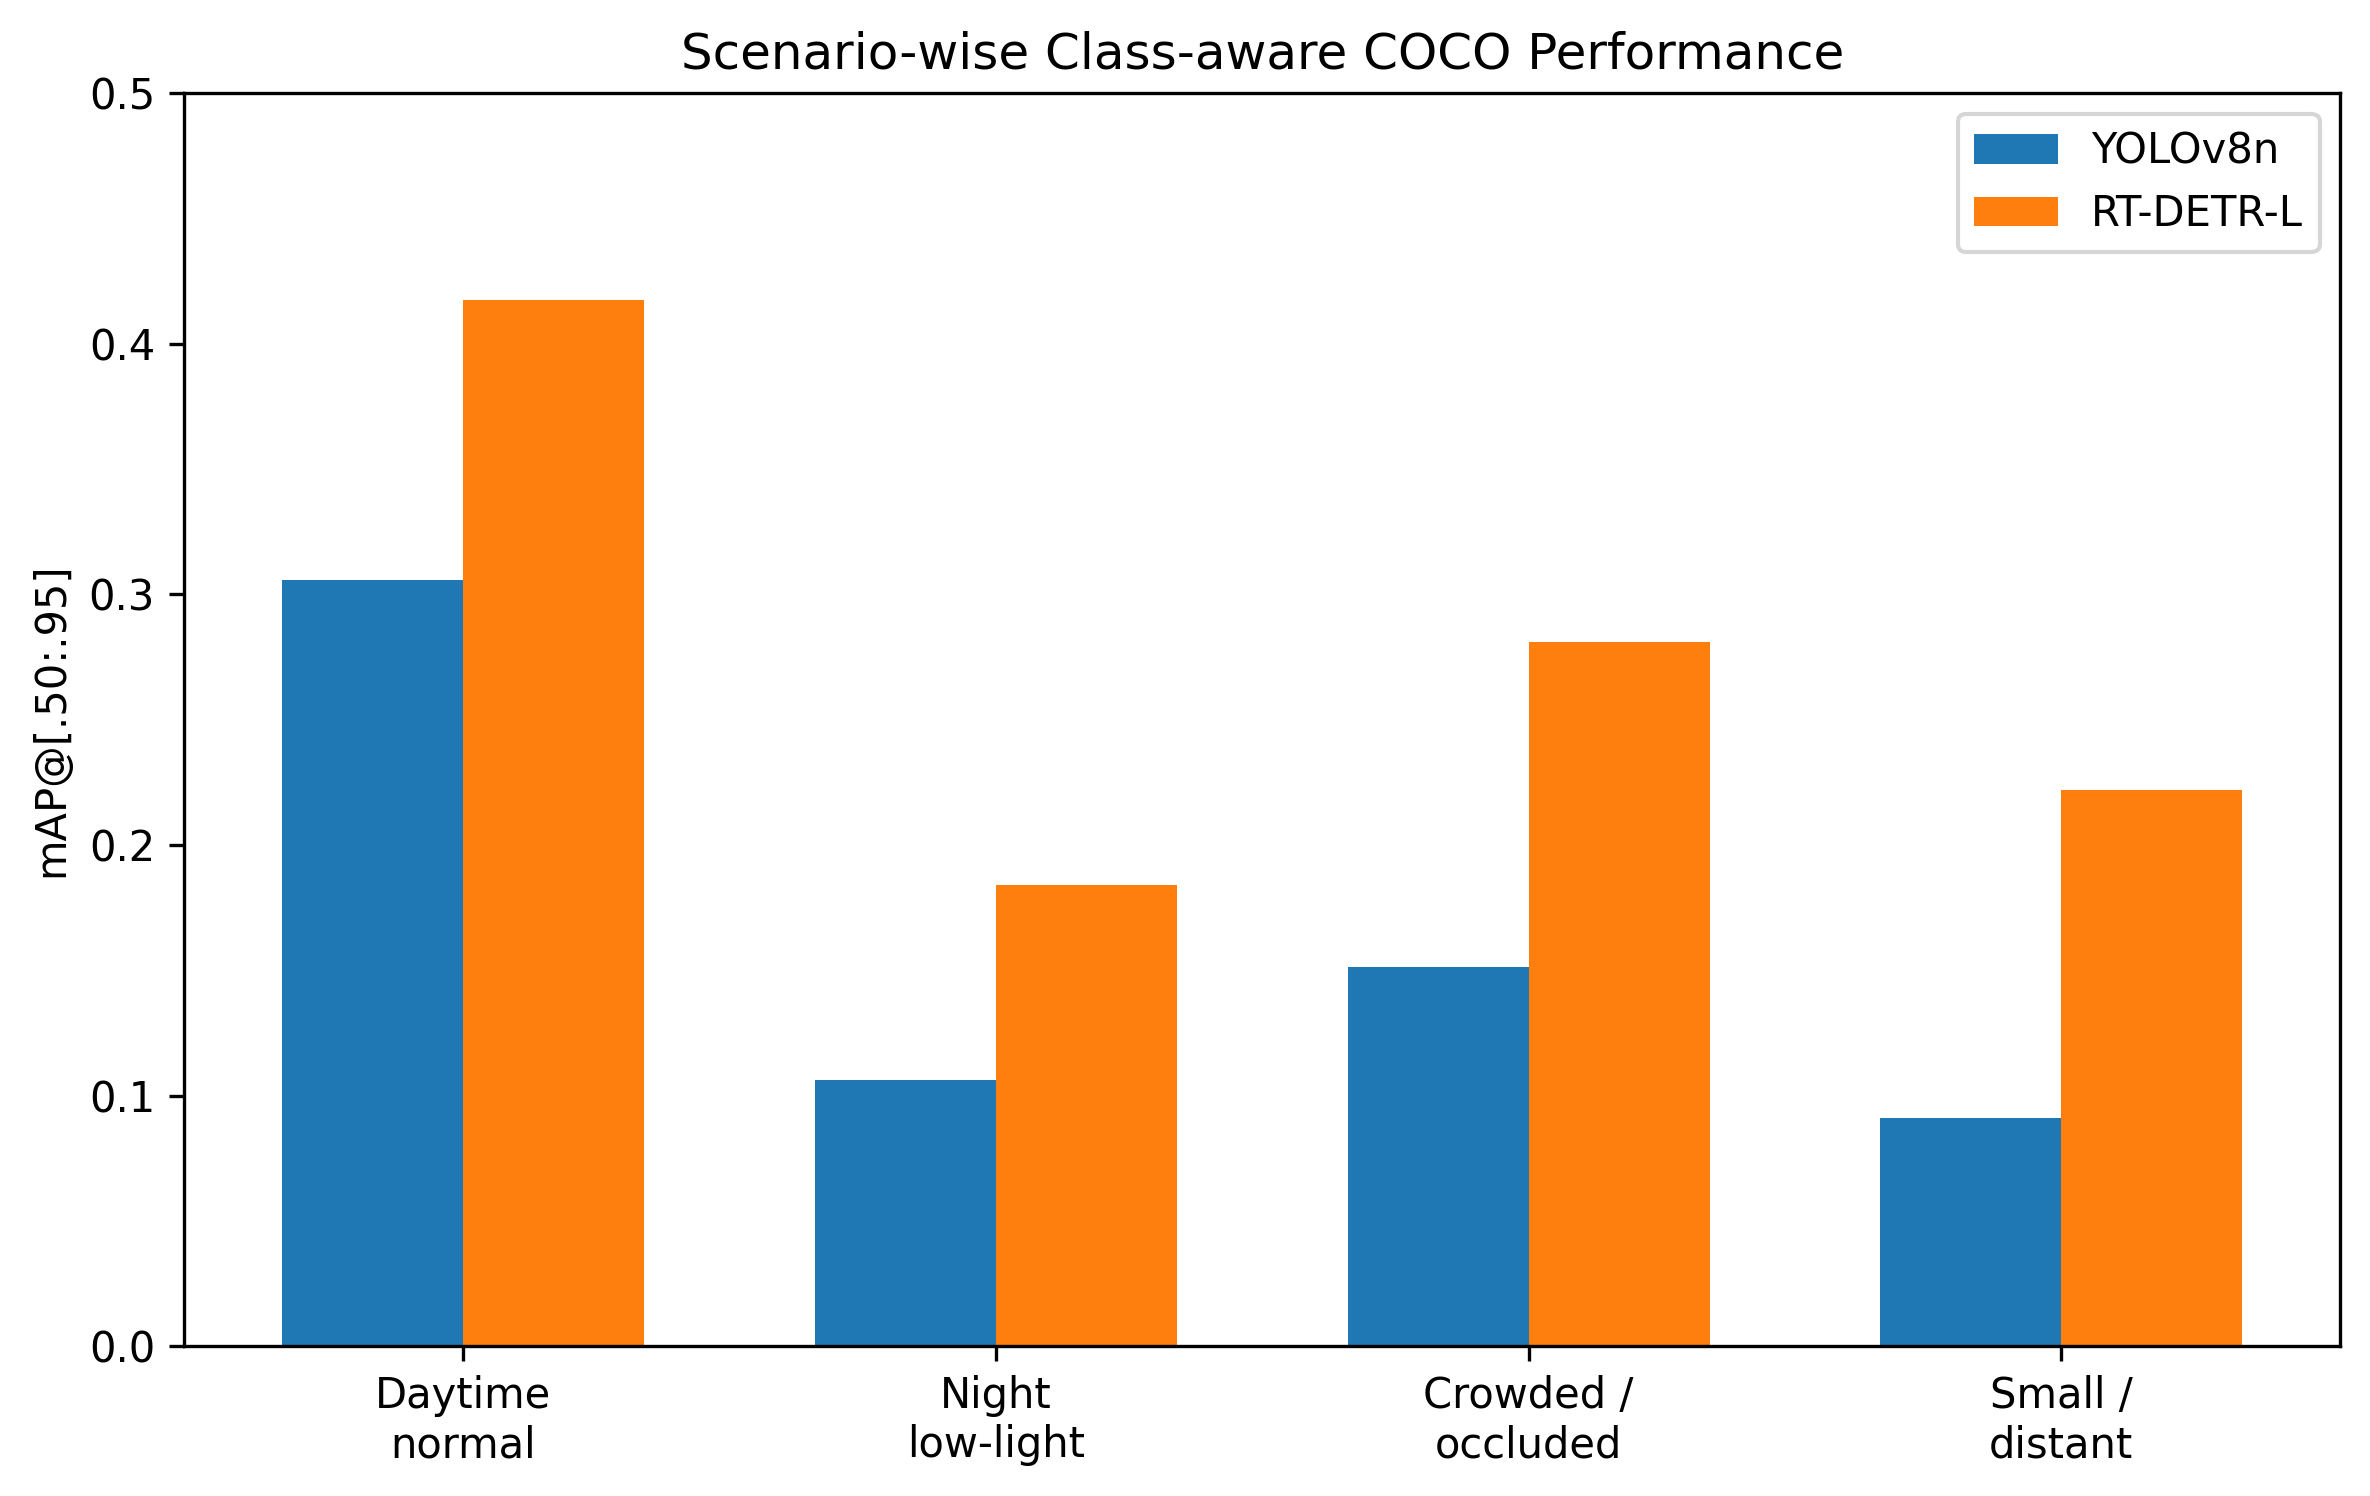
\includegraphics[width=0.84\textwidth]{figures/road200_scenario_map_comparison.png}
\caption{Scenario-wise mAP@[0.50:0.95] on the locked \textsc{Road200} benchmark.}
\label{fig:scenario_map_comparison}
\end{figure}

\FloatBarrier

\begin{table}[H]
\caption{Scenario-wise class-aware results. F1 is calculated at confidence $=0.25$ and IoU $=0.50$.}
\label{tab:scenario_results}
\centering
\small
\begin{tabular}{lrrrr}
\hline
Scenario & YOLO mAP & RT-DETR mAP & YOLO F1 & RT-DETR F1 \\
\hline
Daytime normal & 0.306 & \textbf{0.417} & 0.560 & \textbf{0.647} \\
Night low-light & 0.106 & \textbf{0.184} & 0.315 & \textbf{0.467} \\
Crowded/occluded & 0.151 & \textbf{0.281} & 0.470 & \textbf{0.592} \\
Small/distant & 0.091 & \textbf{0.222} & 0.408 & \textbf{0.565} \\
\hline
\end{tabular}
\end{table}

\subsection{RT-DETR-L Post-processing Ablation}

The post-processing study was performed offline using the frozen RT-DETR-L prediction set. It therefore isolates the effect of confidence filtering, maximum output count, and external class-aware NMS without changing the detector weights or rerunning inference.

Confidence filtering was the dominant factor controlling output density. Raising the confidence floor from 0.001 to 0.35 reduced the average number of retained detections per image from 260.20 to 11.46. This reduction was accompanied by a decrease in mAP from 0.247 to 0.208 and a decrease in recall from 0.832 to 0.518 when each confidence floor was evaluated at its corresponding operating point. At the same time, precision increased from 0.049 to 0.694 and F1 increased from 0.093 to 0.593. Thus, confidence filtering does not provide a free accuracy improvement; it provides an explicit completeness--compactness trade-off.

The maximum-detection sweep had limited influence on the operating-point metrics. Using top-50, top-100, and top-300 predictions produced mAP values of 0.244, 0.246, and 0.247, respectively, while the precision, recall, and F1-score at confidence 0.25 remained unchanged. Consequently, top-100 was retained as a practical safety cap rather than interpreted as an accuracy-improving module.

\begin{figure}[H]
\centering
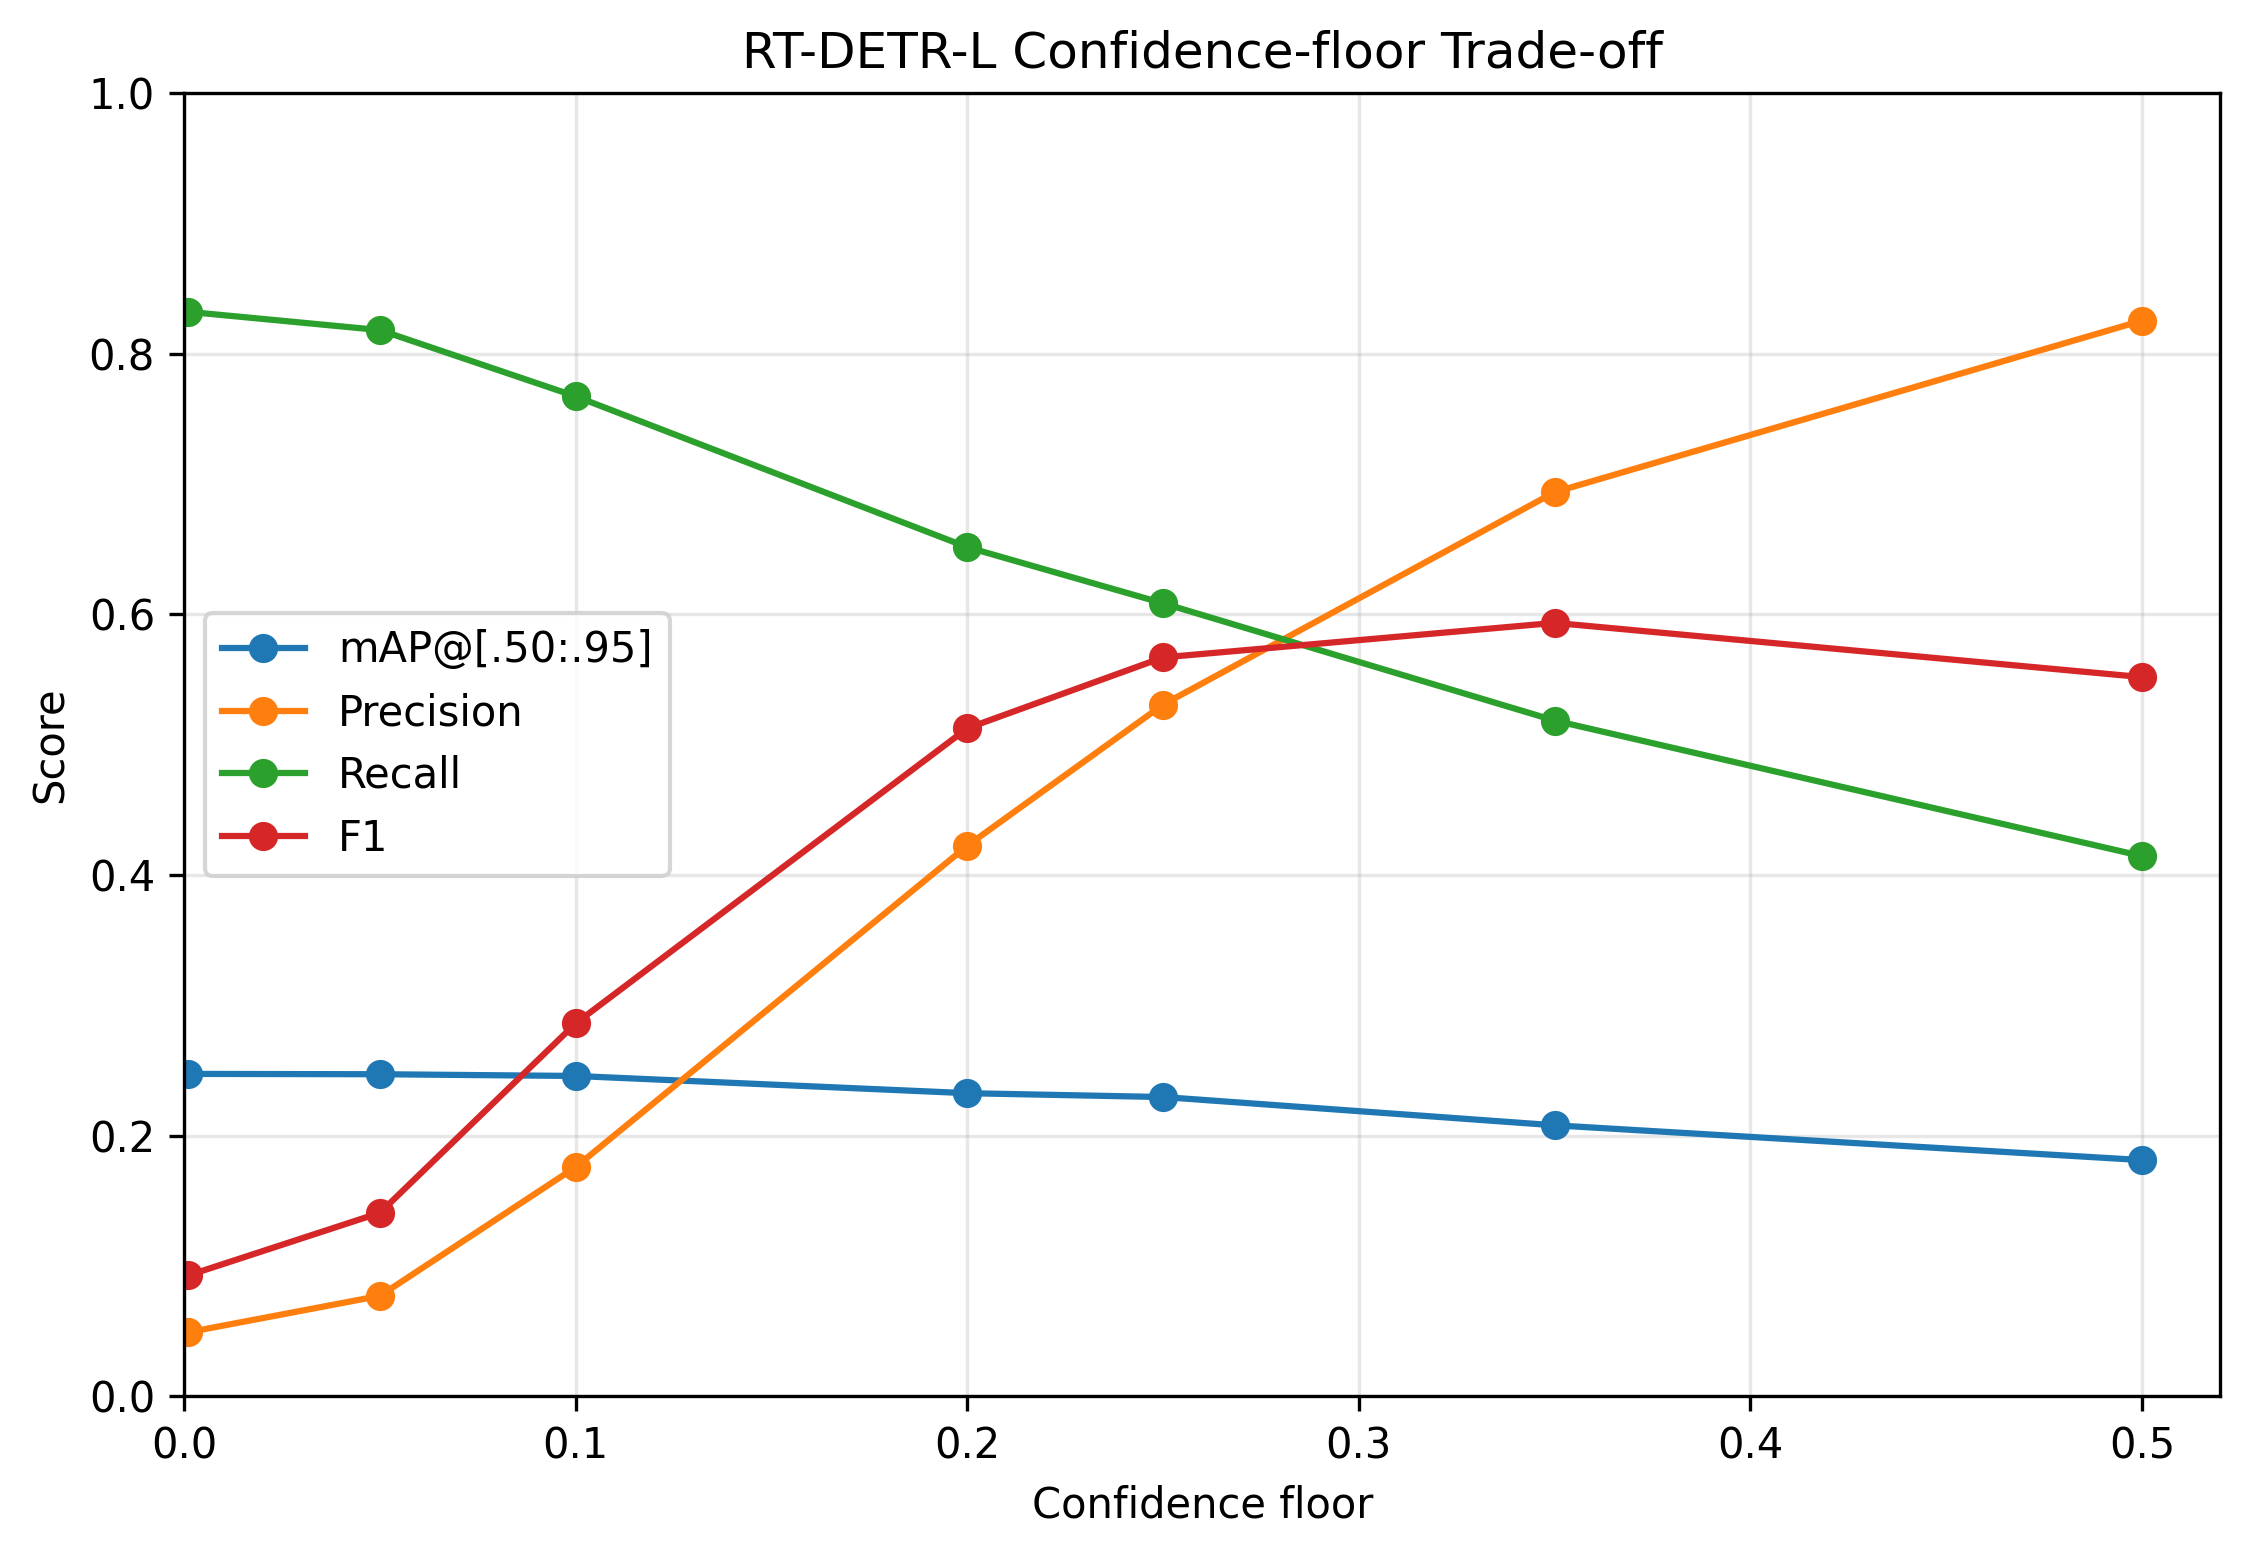
\includegraphics[width=0.82\textwidth]{figures/rtdetr_confidence_tradeoff.png}
\caption{Confidence-floor ablation for RT-DETR-L. Precision, recall, and F1 are calculated at the confidence floor shown on the horizontal axis.}
\label{fig:confidence_ablation}
\end{figure}

External class-aware NMS mainly acted as an output-refinement mechanism. At the raw score floor, NMS with IoU $=0.45$ reduced the average raw output density from 260.20 to 166.65 detections per image and increased the operating-point F1-score from 0.567 to 0.580, while mAP changed from 0.247 to 0.245. NMS with IoU $=0.55$ nearly preserved the baseline mAP (0.247) and produced the highest AP50 value in the NMS sweep (0.460). These changes are modest and should be interpreted as evidence of output refinement rather than as a major improvement in detector accuracy.

Table~\ref{tab:profile_results} compares the three retained RT-DETR-L profiles. The raw metric baseline is used to report standard COCO AP because it preserves the ranked low-confidence prediction tail. The balanced and compact profiles are intended for readable output rather than for replacing the raw mAP baseline. The balanced profile prioritizes recall, while the compact profile provides the highest F1-score and the lowest output density.

\begin{table}[H]
\caption{Final RT-DETR-L output profiles. P, R, and F1 are calculated at the confidence floor of the corresponding profile.}
\label{tab:profile_results}
\centering
\small
\begin{tabular}{lrrrr}
\hline
Profile & mAP & P & R & F1 \\
\hline
Raw metric baseline & \textbf{0.247} & -- & -- & -- \\
Balanced profile & 0.227 & 0.568 & \textbf{0.594} & 0.580 \\
Compact profile & 0.208 & \textbf{0.707} & 0.518 & \textbf{0.598} \\
\hline
\end{tabular}

\vspace{2pt}

\begin{tabular}{lrrr}
\hline
Profile & Confidence & External NMS & Det./image \\
\hline
Raw metric baseline & 0.001 & None & 260.20 \\
Balanced profile & 0.25 & 0.45 & 16.04 \\
Compact profile & 0.35 & 0.55 & 11.23 \\
\hline
\end{tabular}
\end{table}

\FloatBarrier

\subsection{Qualitative Output Analysis}

Figure~\ref{fig:qualitative_crowded} presents the deterministic crowded/occluded qualitative case selected by the procedure described in Section~3.5. The image contains 24 shared-class ground-truth boxes. The raw metric baseline retains 268 ranked candidate detections, which is appropriate for AP calculation but is not suitable as a directly readable visual output. The balanced profile retains 19 detections, while the compact profile retains 16.

The example is consistent with the automatic ablation: thresholding and external class-aware NMS substantially reduce output density. It should not be interpreted as proof that a visually cleaner image is necessarily more accurate. Instead, the example illustrates why the raw AP-ranking output and the deployment-oriented profiles are reported separately. The small/distant qualitative example is retained in the supplementary material because it more clearly demonstrates the potential completeness loss introduced by the compact profile.

\begin{figure}[H]
\centering
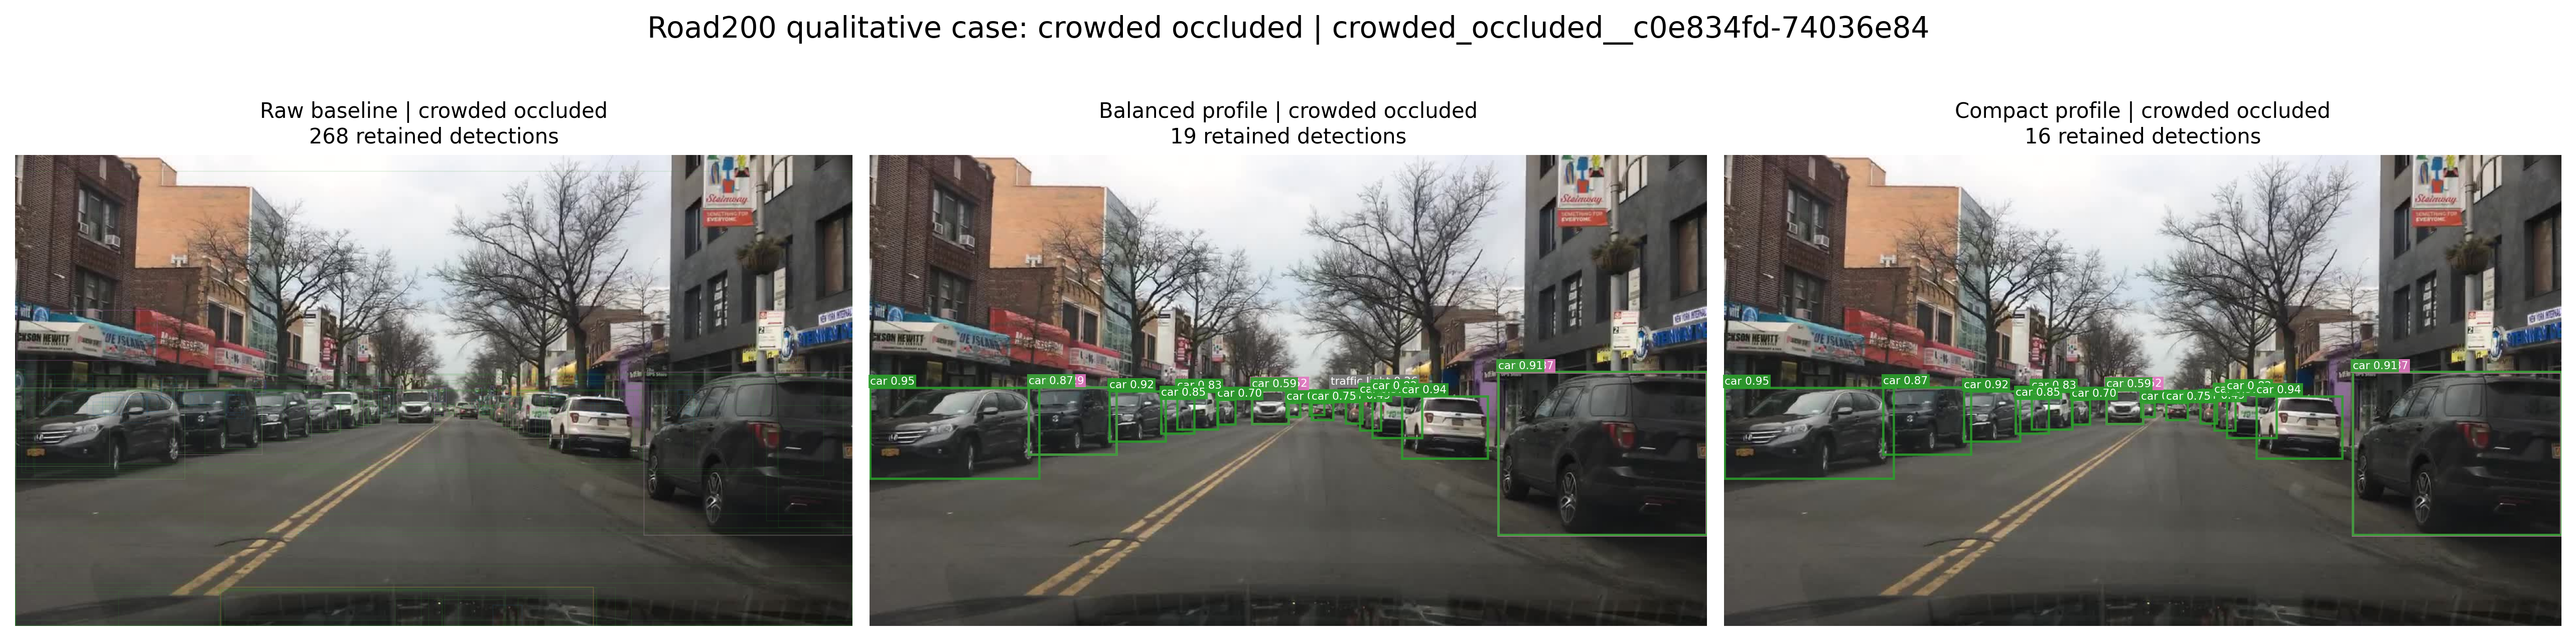
\includegraphics[width=0.98\textwidth]{figures/qualitative_crowded_profiles.png}
\caption{RT-DETR-L output profiles on a deterministically selected crowded/occluded Road200 case. The raw metric baseline retains ranked candidates for AP calculation, whereas the balanced and compact profiles are deployment-oriented output configurations.}
\label{fig:qualitative_crowded}
\end{figure}

\FloatBarrier

\section{Discussion}

\subsection{Detector-level Interpretation}

The standardized \textsc{Road200} evaluation changes the interpretation of the model comparison from an output-count observation to a ground-truth-based result. RT-DETR-L achieved higher class-aware mAP@[0.50:0.95], AP50, AP75, recall, and F1-score than YOLOv8n on the locked benchmark, whereas YOLOv8n achieved higher precision at the common operating threshold. Therefore, the practical distinction between the two detectors in this study is not adequately described as a simple speed--accuracy trade-off. Instead, the results show a precision--completeness trade-off at the selected operating point.

YOLOv8n produced a more conservative set of detections at confidence 0.25. This behaviour led to fewer false positive predictions relative to its retained outputs, but also to substantially lower recall. RT-DETR-L retained more valid objects under the same class-aware matching protocol, resulting in a higher F1-score and stronger COCO AP metrics. These findings are consistent with the motivation for evaluating Transformer-based detectors in difficult road scenes, but this study does not isolate an architectural causal mechanism. In particular, the experiment does not prove that global attention alone caused the observed difference; it establishes only that the pretrained RT-DETR-L model produced stronger measured results on the locked \textsc{Road200} benchmark.

The class-level results provide an additional qualification. The RT-DETR-L advantage was not limited to the dominant \texttt{car} category, but was also observed for \texttt{person} and \texttt{traffic light}, which are more sensitive to scale, occlusion, and visual ambiguity in road scenes. At the same time, categories with very few instances should not be over-interpreted. The \texttt{train} category had no ground-truth instance in \textsc{Road200}, while bicycle and motorcycle instances were sparse. The principal evidence should therefore be understood as an aggregate result over the shared taxonomy rather than as a definitive category-specific benchmark.

\subsection{Scenario-dependent Implications}

The scenario breakdown shows that the overall advantage of RT-DETR-L was not uniformly distributed. The largest absolute mAP gains occurred in the small/distant and crowded/occluded groups. This is practically relevant because these conditions are associated with two common road-scene difficulties: limited visible object extent and overlapping objects within dense traffic layouts.

However, the scenario results should not be interpreted as evidence that RT-DETR-L solves these problems. Both detectors experienced lower performance under night low-light conditions, and both remained less effective on small or distant objects than in daytime normal scenes. The appropriate conclusion is therefore comparative rather than absolute: RT-DETR-L retained a larger performance margin over YOLOv8n in the evaluated small/distant and crowded/occluded subsets, while difficult illumination remained a shared challenge.

This distinction matters for deployment-oriented interpretation. A detector that performs well in daytime normal traffic may still require conservative downstream handling when visibility is reduced. Conversely, the higher recall observed for RT-DETR-L in crowded and small-object scenes may be useful when missing road users has a higher practical cost than presenting some additional candidate boxes. The choice between detector outputs should therefore depend on the relative priority assigned to completeness, false-positive control, and human or downstream-system capacity to process detections.

\subsection{What Post-processing Improves}

The post-processing ablation shows that confidence filtering is the principal control variable for output density. Raising the confidence floor substantially reduced the number of displayed detections per image and increased precision, but it also reduced recall and COCO AP. This confirms that a visually cleaner output is not equivalent to a more accurate detector. The compact profile is useful when concise output and false-positive control are prioritized, but it deliberately discards some candidate detections and should not replace the raw ranked predictions used for standard AP calculation.

The external class-aware NMS study provides a narrower conclusion. External NMS did not materially change strict mAP@[0.50:0.95], but it modestly improved operating-point precision and F1-score while reducing redundant outputs. Its contribution is therefore best described as output refinement rather than accuracy enhancement. This is also why the method is explicitly labelled as \emph{external class-aware NMS}: RT-DETR-L is an end-to-end detector family and the study does not claim that conventional NMS is a native requirement of the model.

The final profiles provide two distinct deployment-oriented options. The balanced profile retains more detections and achieves the stronger recall-oriented behaviour, making it suitable when completeness is prioritised. The compact profile produces fewer retained detections per image and the highest F1-score among the selected profiles, making it suitable when readability and precision are more important. Reporting both profiles is more transparent than selecting one configuration as universally optimal, because the two profiles encode different operating priorities.

\subsection{Scope and Limitations}

The conclusions are bounded by the design of \textsc{Road200}. The benchmark is a reproducible 200-image case-study subset rather than a replacement for a large-scale road-scene benchmark. All images originate from the BDD100K validation split, and only eight BDD100K-to-COCO compatible categories were included in automatic evaluation. Consequently, the results should not be generalized to every road-scene category, every geographical setting, or every weather condition.

The study compares two pretrained detectors without fine-tuning on \textsc{Road200}. It therefore evaluates the practical behaviour of publicly available pretrained outputs rather than the maximum attainable performance of either model after domain-specific training. In addition, the standardized evaluation loop includes image loading, prediction conversion, and metric export. It was designed for reproducible detection evaluation rather than a dedicated latency benchmark. Claims about real-time deployment latency would require a separate controlled experiment with explicit warm-up, batch-size, preprocessing, and timing procedures.

Finally, the post-processing experiments were conducted on frozen RT-DETR-L predictions. This allows the influence of confidence filtering, top-$K$ capping, and external class-aware NMS to be isolated without retraining or re-running inference. It does not establish that the same parameter settings will be optimal for other RT-DETR variants, different datasets, or systems with different safety requirements. Future work should test the same protocol across additional DETR-family models, broader annotated road-scene data, and controlled end-to-end deployment settings.

\FloatBarrier

\section{Conclusion}

This paper presented a reproducible empirical study of pretrained YOLOv8n and RT-DETR-L outputs on \textsc{Road200}, a locked 200-image road-scene subset derived from the BDD100K validation split. The benchmark combines four scenario groups---daytime normal, night low-light, crowded/occluded, and small/distant---with official BDD100K \texttt{box2d} annotations and an explicit eight-class BDD100K-to-COCO mapping. This design enabled standard class-aware COCO evaluation while preserving a scenario-oriented analysis of practical road-scene difficulties.

On the locked benchmark, RT-DETR-L achieved stronger automatic detection results than YOLOv8n, obtaining an mAP@[0.50:0.95] of 0.247 compared with 0.127 for YOLOv8n. RT-DETR-L also achieved higher AP50, AP75, recall, and F1-score at the specified operating point, whereas YOLOv8n retained higher precision. The scenario analysis showed that the relative RT-DETR-L advantage was especially pronounced in the crowded/occluded and small/distant groups. Nevertheless, both detectors experienced substantial degradation under night low-light conditions, indicating that difficult illumination remains an unresolved challenge.

The post-processing experiments showed that output usability should be treated separately from raw detection capability. Confidence filtering was the dominant control variable for output density: higher thresholds produced substantially fewer retained detections and higher precision, but reduced recall and COCO AP. External class-aware NMS modestly reduced redundant outputs and improved operating-point F1 in some configurations, while producing little change in strict COCO mAP. Accordingly, this paper distinguishes between the raw metric baseline used for standard AP calculation and two deployment-oriented profiles: a balanced profile that retains more detections and a compact profile that prioritizes precision, F1-score, and visual readability. These profiles are not claimed to improve the underlying RT-DETR-L architecture; they provide transparent output-level choices for different completeness--compactness priorities.

The study is limited to a 200-image case-study benchmark, two pretrained detectors, and frozen RT-DETR-L predictions. Future work should extend the protocol to broader annotated road-scene data, additional DETR-family architectures, and controlled end-to-end deployment measurements with dedicated latency and resource profiling. It would also be valuable to evaluate scenario-adaptive output thresholds and to investigate whether learned confidence calibration or task-specific fine-tuning can improve small-object and night-time detection without sacrificing output usability.

\subsubsection*{Acknowledgements}
The authors thank the module teaching team and colleagues who provided constructive feedback during the development of this work.

\bibliographystyle{splncs04}
\bibliography{references}

\end{document}
